\documentclass{article}

% Packages
\usepackage{amsmath} % for math
\usepackage{geometry} % for page margins
\usepackage{graphicx} % for images
\usepackage{hyperref} % for content table
\usepackage{float} % for figure positioning
\usepackage{indentfirst} % for indenting the first paragraph
\usepackage{listings} % for code blocks
\usepackage{xcolor} % for setting colors

% Define the colors for your code block
\definecolor{codegreen}{rgb}{0,0.6,0}
\definecolor{codegray}{rgb}{0.5,0.5,0.5}
\definecolor{codepurple}{rgb}{0.58,0,0.82}
\definecolor{backcolour}{rgb}{0.95,0.95,0.92}

% Define the settings for your code block
\lstdefinestyle{mystyle}{
    backgroundcolor=\color{backcolour},
    commentstyle=\color{codegreen},
    keywordstyle=\color{magenta},
    numberstyle=\tiny\color{codegray},
    stringstyle=\color{codepurple},
    basicstyle=\ttfamily\footnotesize,
    breakatwhitespace=false,
    breaklines=true,
    captionpos=b,
    keepspaces=true,
    numbers=left,
    numbersep=5pt,
    showspaces=false,
    showstringspaces=false,
    showtabs=false,
    tabsize=2
}

\lstset{style=mystyle}

% Title and author
\title{Projet \texttt{minishell} - Rapport}
\author{Vianney HERVY - 1ASN Groupe H}

\begin{document}

\maketitle
\tableofcontents
\newpage

\section{Architecture}

L'architecture de ce projet est simple étant donné qu'elle nous est presque imposée par le sujet. La majorité du code utile sur trouve dans le fichier \texttt{minishell.c}. Le package formé par \texttt{readcmd.c} et \texttt{readcmd.h} est utilisé pour extraire de la commande utilisateur les informations telles que la mise en arrière plan, les redirections, les tubes etc.

\section{Choix et spécificités de conception}

J'ai rapidement vu que la gestion d'erreur en C n'était pas une mince affaire. Pour éviter kes répétitions de code, j'ai créé 5 fonctions "sûres" qui gèrent les erreurs de manière uniforme. Ces fonctions sont \texttt{safeopen}, \texttt{safeclose}, \texttt{safedup2}, \texttt{safeexecvp} et \texttt{safepipe}.

\begin{lstlisting}[language=C, caption=Code des fonctions "sûres"]
/* Ouvrir le fichier `nom` dans un descripteur de fichier en assurant la bonne execution. Retourne le descripteur de fichier associe. */
int safeopen(char *nom, int flags, mode_t mode) {
    int desc_open;
    if (mode) {
        desc_open = open(nom, flags, mode);
    } else {
        desc_open = open(nom, flags);
    }
    if (desc_open == -1) {
        fprintf(stderr, "Erreur a l'ouverture de %s", nom);
        exit(EXIT_FAILURE);
    }
    return desc_open;
}

/* Fermer le fichier de descripteur `desc` en verifiant la bonne fermeture. `nom` est utilise en cas d'erreur. */
void safeclose(int desc, char *nom) {
    int desc_close = close(desc);
    if (desc_close == -1) {
        fprintf(stderr, "Erreur a la fermeture du descripteur %s", nom);
        exit(EXIT_FAILURE);
    }
}

/* Dupliquer (cf `dup2`) en assurant la bonne execution. `nom` est utlise en cas d'erreur. */
void safedup2(int oldfd, int newfd, char *nom) {
    if (dup2(oldfd, newfd) == -1) {
        fprintf(stderr, "Erreur au dup %s", nom);
        exit(EXIT_FAILURE);
    }
}

/* Executer `cmd0` avec `execvp` en s'assurant de la bonne execution. */
void safeexecvp(char *cmd0, char *const argv[]) {
    if (execvp(cmd0, argv) == -1) {
        fprintf(stderr, "Commande inconnue : %s", cmd0);
        exit(EXIT_FAILURE);
    }
}

/* Creer un tube en s'assurant du succes de l'operation */
void safepipe(int tube[2]) {
    if (pipe(tube) == -1) {
        perror("Erreur lors de la creation du tube");
        exit(EXIT_FAILURE);
    }
}
\end{lstlisting}

Dans les listings, je pourrais ne pas montrer ces processus de gestion d'erreur afin de garder un code concis. Toutefois, je les ai utilisé autant que possible dans le code de mon projet.

\section{Méthodologie des tests}

Pour les étapes où des changements majeurs sont apportés au code, jai pris soin de vérifier que toutes les fonctionnalités précédentes fonctionnaient toujours. Par exemple, après l'étape 20, j'ai vérifié que les redirections classiques (\texttt{cmd < file} et \texttt{cmd > file}) étaient bien effectuées. De même, j'ai testé que les redirections et pipelines en arrière plan fonctionnaient correctement.

\section{Étapes}

\subsection*{Étape 1 (Testez le programme)}
\addcontentsline{toc}{subsection}{Étape 1 (Testez le programme)}

\begin{figure}[H]
    \centering
    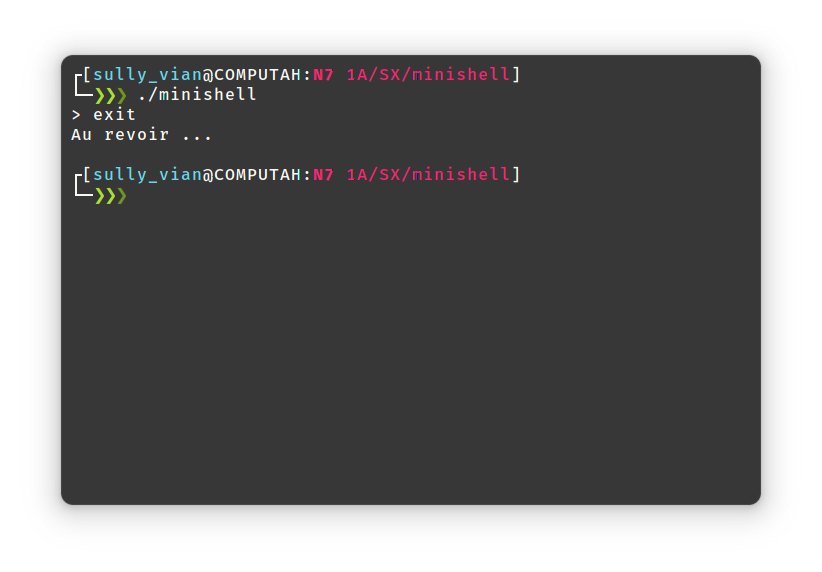
\includegraphics[width=1\textwidth]{./resources/E1.png}
    \caption{Test du programme}
\end{figure}

\subsection*{Étape 2 (Lancement d'une commande)}
\addcontentsline{toc}{subsection}{Étape 2 (Lancement d'une commande)}

C'est le fils qui exécute la commande.

\begin{lstlisting}[language=C, caption=Code de la question 2]
/* ... */
case 0: /* code du fils */
    execvp(cmd[0], cmd);
    break;
/* ... */
\end{lstlisting}

Sur la figure 3, on voit un exemple de recouvrement: le processus père, responsable de l'affichage du prompt, n'attend pas la terminaison du fils (ici la commande \texttt{ls}) pour écrire \texttt{>}.

\begin{figure}[H]
    \centering
    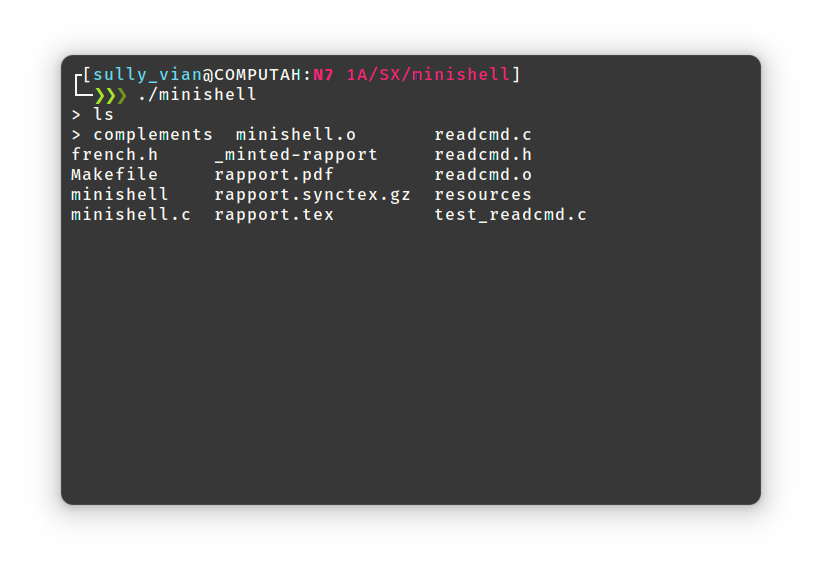
\includegraphics[width=1\textwidth]{./resources/E2.png}
    \caption{Exemple du lancement de la commande \texttt{ls}}
\end{figure}

\subsection*{Étape 3 (Enchaînement séquentiel des commandes)}
\addcontentsline{toc}{subsection}{Étape 3 (Enchaînement séquentiel des commandes)}

Pour que le père attende la terminaison du fils, il suffit d'ajouter la commande bloquante \texttt{wait(null)} dans le code du père tel qu'indiqué dans le listing 1.

\begin{lstlisting}[language=C, caption=Ajout pour la question 3]
/* ... */
default: /* code du pere */
    wait(null); // attendre terminaison du fils
    break;
/* ... */
\end{lstlisting}

La figure 3 montre un exemple de lancement de la commande \texttt{ls} avec un père patient.

\begin{figure}[H]
    \centering
    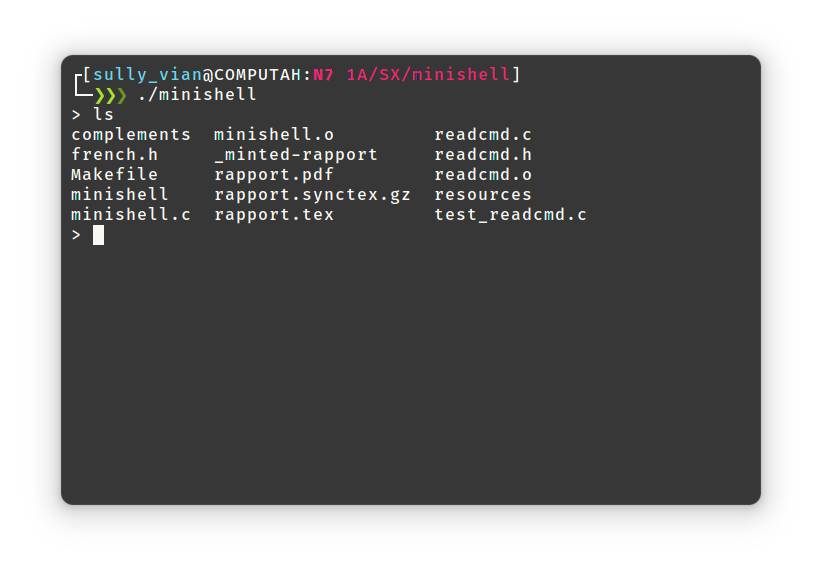
\includegraphics[width=1\textwidth]{./resources/E3.png}
    \caption{Exemple du lancement de la commande \texttt{ls} avec un père patient}
\end{figure}

\subsection*{Étape 4 (Lancement de commandes en tâche de fond)}
\addcontentsline{toc}{subsection}{Étape 4 (Lancement de commandes en tâche de fond)}

Pour ne pas attendre la terminaison d'un fils mis en arrière plan, il suffit de vérifier si le champ \texttt{backgrounded} de la structure \texttt{commande} est \texttt{NULL}. Si c'est le cas, ola commande est en avant plan et on l'attend comme implémenté dans le listing 2.

\begin{lstlisting}[language=C, caption=Ajout pour la question 4]
default: /* code du pere */
    if (commande->backgrounded == NULL) {
        // on n'attend pas la terminaison d'un fils mis en arriere plan
        wait(null);
    }
\end{lstlisting}

Pour vérifier que le père n'attend pas la terminaison d'un fils en arrière plan, on peut lancer la commande \texttt{sleep 5 \&} et voir que le prompt est affiché directement, sans attendre avant la fin du sommeil.

\subsection*{Étape 5 (Rendu)}
\addcontentsline{toc}{subsection}{Étape 5 (Rendu)}

Rien à faire.

\subsection*{Étape 6 (Traitement du signal \texttt{SIGCHLD})}
\addcontentsline{toc}{subsection}{Étape 6 (Traitement du signal \texttt{SIGCHLD})}

\begin{lstlisting}[language=C, caption=ajout de la question 6]
/* ... */
void traitement(int sig) {
    switch (sig) {
        case SIGCHLD:
            printf("Un fils vient de se terminer\n");
            break;
        default:
            printf("Signal inconnu\n");
            break;
    }
}
/* ... */
int main(void) {
    struct sigaction action;
    action.sa_handler = traitement;
    sigemptyset(&action.sa_mask);
    action.sa_flags = SA_RESTART;
    sigaction(SIGCHLD, &action, NULL);
}
/* ... */
\end{lstlisting}

\subsection*{Étape 7 (Utilisation de \texttt{SINGINT} pour traiter la terminaison des processus fils)}
\addcontentsline{toc}{subsection}{Étape 7 (Utilisation de \texttt{SINGINT} pour traiter la terminaison des processus fils)}

\begin{lstlisting}[language=C, caption=ajout de la question 7]
/* ... */
void traitement(int sig) {
    pid_t pid;
    switch (sig) {
        case SIGCHLD:
            pid = waitpid(-1, NULL, WNOHANG | WUNTRACED | WCONTINUED);
            printf("sortie du processus de pid = %d\n", pid);
            break;
        default:
            printf("Signal inconnu\n");
            break;
    }
}
/* ... */
\end{lstlisting}

\subsection*{Étape 8 (Attendre un signal : \texttt{pause})}
\addcontentsline{toc}{subsection}{Étape 8 (Attendre un signal : \texttt{pause})}

\begin{lstlisting}[language=C, caption=ajout de la question 8]
/* ... */
default: /* code du pere */
    pause(); // attendre un signal
    break;
/* ... */
\end{lstlisting}

\begin{figure}[H]
    \centering
    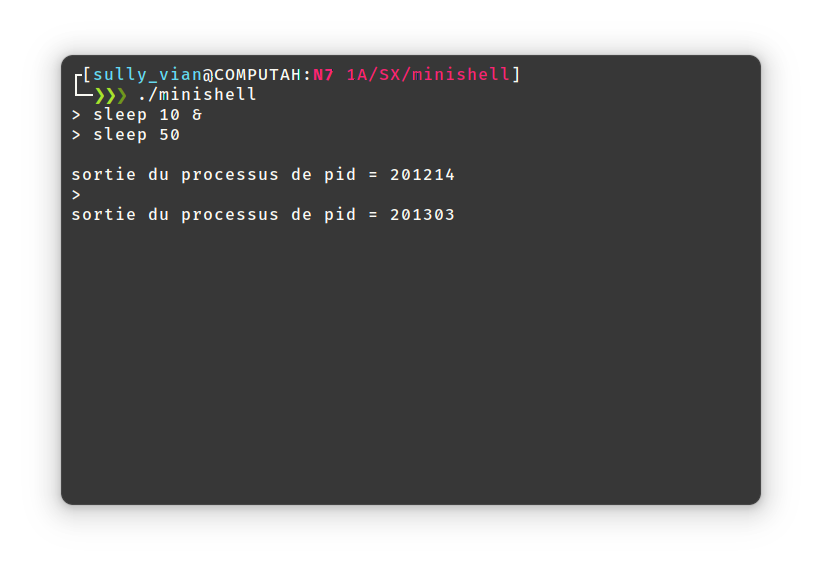
\includegraphics[width=\textwidth]{./resources/E8.png}
    \caption{Démonstration de la terminaison en arrière plan du premier \texttt{sleep}}
\end{figure}

\subsection*{Étape 9 (Suspension et reprise d'un processus en arrière plan)}
\addcontentsline{toc}{subsection}{Étape 9 (Suspension et reprise d'un processus en arrière plan)}

Lors de l'envoi du signal \texttt{SIGSTOP} à un processus en arrière plan, ce processus est mis en pause et passe à l'état "stopped". Lors de l'envoi du signal \texttt{SIGCONT}, le processus reprend son exécution et passe de nouveau à l'état "running".

\subsection*{Étape 10 (Affichage d'un message indiquant le signal reçu)}
\addcontentsline{toc}{subsection}{Étape 10 (Affichage d'un message indiquant le signal reçu)}

\begin{lstlisting}[language=C, caption=ajout de la question 10]
/* ... */
void traitement(int sig) {
    pid_t pid;
    switch (sig) {
        case SIGCHLD:
            pid = waitpid(-1, null, WNOHANG | WUNTRACED | WCONTINUED);

            if (WIFEXITED(status)) {
                printf("\nsortie du processus de pid = %d\n", pid);
            }
            if (WIFSIGNALED(status)) {
                printf("\nterminaison du processus de pid = %d par le signal %d\n", pid, sig);
            }
            if (WIFSTOPPED(status)) {
                printf("\ninterruption du processus de pid = %d\n", pid);
            }
            if (WIFCONTINUED(status)) {
                printf("\nreprise du processus de pid = %d\n", pid);
            }
            break;

        default:
            printf("autre signal\n");
            break;
    }
}
/* ... */
\end{lstlisting}

\subsection*{Étape 11 (Rendu)}
\addcontentsline{toc}{subsection}{Étape 11 (Rendu)}

Rien à faire.

\subsection*{Étape 12 (Test de la frappe au clavier de \texttt{ctrl-c} et \texttt{ctrl-z})}
\addcontentsline{toc}{subsection}{Étape 12 (Test de la frappe au clavier de \texttt{ctrl-c} et \texttt{ctrl-z})}

Lorsque le \texttt{minishell} est lancé, les signaux \texttt{SIGINT} et \texttt{SIGTSTP} causent l'arrêt du processus père ainsi que celui de chacun de ses fils.

\subsection*{Étape 13 (Gestion de la frappe au clavier de \texttt{ctrl-c} et \texttt{ctrl-z})}
\addcontentsline{toc}{subsection}{Étape 13 (Gestion de la frappe au clavier de \texttt{ctrl-c} et \texttt{ctrl-z})}

\subsubsection*{Étape 13.1 (Changer le traitement des signaux \texttt{SIGINT} et \texttt{SIGTSTP})}
\addcontentsline{toc}{subsubsection}{Étape 13.1 (Changer le traitement des signaux \texttt{SIGINT} et \texttt{SIGTSTP})}

\begin{lstlisting}[language=C, caption=ajout de la question 13.1]
/* ... */
void traitement(int sig) {
    switch (sig) {
        case SIGINT:
            printf("\n[SIGINT]\n");
            break;

        case SIGTSTP:
            printf("\n[SIGSTP]\n");
            break;
/* ... */
}
\end{lstlisting}

\begin{figure}[H]
    \centering
    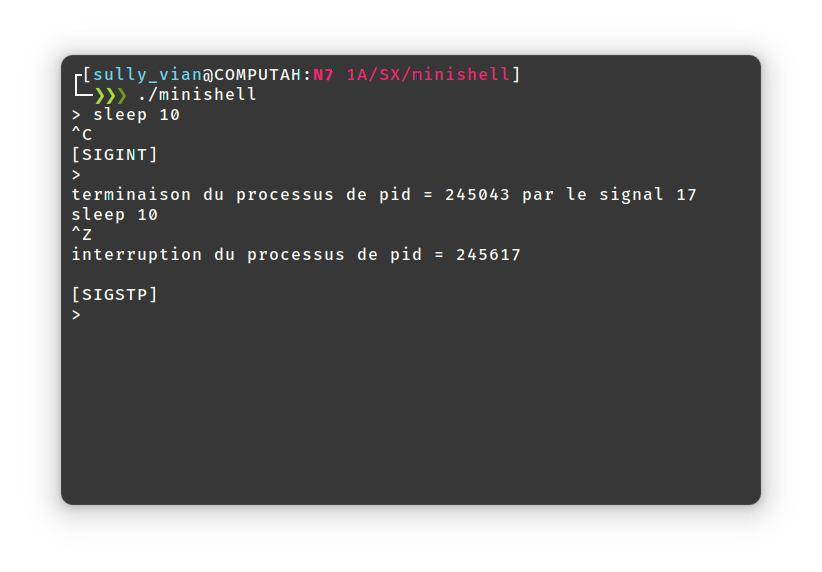
\includegraphics[width=\textwidth]{./resources/E13.1.png}
    \caption{Test de la frappe au clavier de \texttt{ctrl-c} et \texttt{ctrl-z}}
\end{figure}

\subsubsection*{Étape 13.2 (Ignorer les signaux \texttt{SIGINT} et \texttt{SIGTSTP})}
\addcontentsline{toc}{subsubsection}{Étape 13.2 (Ignorer les signaux \texttt{SIGINT} et \texttt{SIGTSTP})}

\subsubsection*{Étape 13.3 (Masquer les signaux \texttt{SIGINT} et \texttt{SIGTSTP})}
\addcontentsline{toc}{subsubsection}{Étape 13.3 (Masquer les signaux \texttt{SIGINT} et \texttt{SIGTSTP})}

\begin{lstlisting}[language=C, caption=ajout de la question 13.3]
    int main(void) {
        /* ... */
        sigset_t mask;
        sigemptyset(&mask);
        sigaddset(&mask, SIGINT);
        sigaddset(&mask, SIGTSTP);
        sigprocmask(SIG_BLOCK, &mask, NULL);
        /* ... */
    }
\end{lstlisting}

Sur la figure 6, on voit que le \texttt{minishell} ne réagit plus aux signaux \texttt{SIGINT} et \texttt{SIGTSTP}.

\begin{figure}[H]
    \centering
    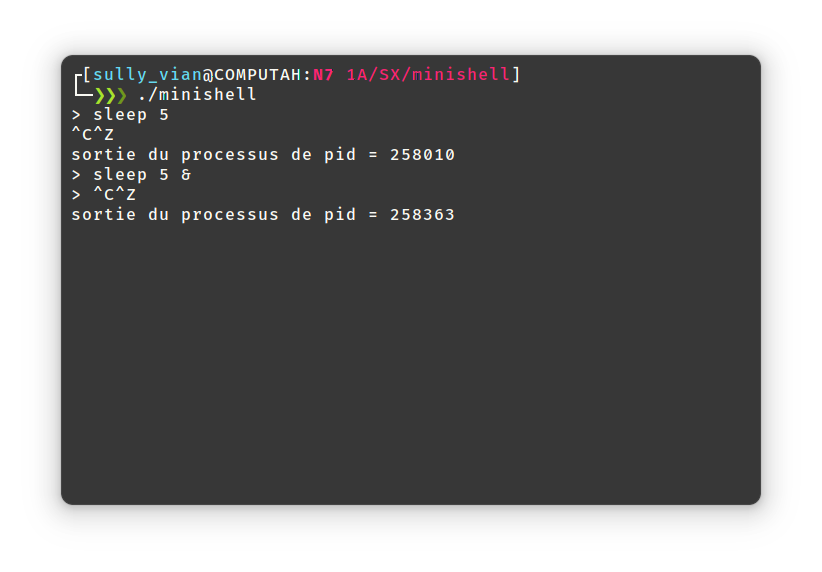
\includegraphics[width=\textwidth]{./resources/E13.3.png}
    \caption{Test de la frappe au clavier de \texttt{ctrl-c} et \texttt{ctrl-z}}
\end{figure}

\subsection*{Étape 14 (Détacher les processus fils en arrière plan)}
\addcontentsline{toc}{subsection}{Étape 14 (Détacher les processus fils en arrière plan)}

En enlevant le masquage réalisé juste au dessus (je l'ai commenté dans mon code) et en détachant les processus fils en arrière plan (à l'aide de \texttt{setpgrp}), les signaux \texttt{SIGINT} et \texttt{SIGTSTP} n'ateignent plus le processus père et ses fils en arrière plan.

\begin{lstlisting}[language=C, caption=ajout de la question 14]
/* ... */
case 0: /* code du fils */
    if (commande->backgrounded != NULL) {
        // changer de groupe si en arriere plan
        setpgrp();
    }
/* ... */
\end{lstlisting}

Dans la figure 7, on voit qu'un processus en avant plan est interrompu mais qu'un processus en arrière plan n'est pas affecté par les signaux \texttt{SIGINT} et \texttt{SIGTSTP}. Le \texttt{minishell}, lui, continue de fonctionner normalement.

\begin{figure}[H]
    \centering
    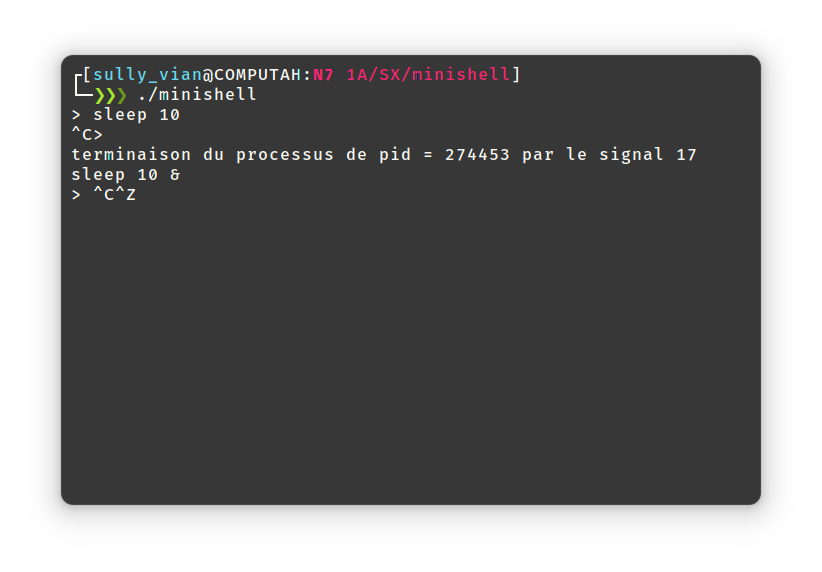
\includegraphics[width=\textwidth]{./resources/E14.png}
    \caption{Test de la frappe au clavier de \texttt{ctrl-c} et \texttt{ctrl-z}}
\end{figure}

\subsection*{Étape 15 (Rendu)}
\addcontentsline{toc}{subsection}{Étape 15 (Rendu)}

Rien à faire.

\subsection*{Étape 16 (Redirections)}
\addcontentsline{toc}{subsection}{Étape 16 (Redirections)}

Pour cette étape, il faut ajouter à la fois la gestion d'entrée et de sortie. Ces deux étapes sont similaires, il suffit de remplacer le descripteur de fichier standard d'entrée (\texttt{STDIN\_FILENO}) par le descripteur du fichier d'entrée et le descripteur de sortie standard (\texttt{STDOUT\_FILENO}) par le descripteur du fichier de sortie.

Dans les deux cas, il faut :
\begin{enumerate}
    \item ouvrir le fichier avec \texttt{open}
    \item dupliquer le descripteur de fichier sur celui voulu (entrée / sortie) avec \texttt{dup2}
    \item fermer le descripteur de fichier ouvert avec \texttt{close}
\end{enumerate}
À chacune de ces étapes, on vérifie que l'opération s'est bien déroulée pour éviter les mauvaises surprises.

\begin{lstlisting}[language=C, caption=gestion des redirections]
case 0: /* code du fils */
    /* ... */
    /* remplacer l'entree standard par commande->in */
    char *in = commande->in;
    if (in != NULL) { /* cmd < file */
        int in_desc;
        if ((in_desc = open(in, O_RDONLY)) == -1) {
            fprintf(stderr, "Erreur a l'ouverture de %s", in);
            exit(EXIT_FAILURE);
        }
        if (dup2(in_desc, STDIN_FILENO) == -1) {
            fprintf(stderr, "Erreur au dup in");
            exit(EXIT_FAILURE);
        }
        if (close(in_desc) == -1) {
            fprintf(stderr, "Erreur a la fermeture du descripteur in");
            exit(EXIT_FAILURE);
        }
    }

    /* remplacer la sortie standard par commande->out */
    char *out = commande->out;
    if (out != NULL) { /* cmd > file */
        int out_desc;
        if ((out_desc = open(out, O_WRONLY|O_CREAT|O_TRUNC, 0644)) == -1) {
            fprintf(stderr, "Erreur a l'ouverture de %s", out);
            exit(EXIT_FAILURE);
        }
        if (dup2(out_desc, STDOUT_FILENO) == -1) {
            fprintf(stderr, "Erreur au dup out");
            exit(EXIT_FAILURE);
        }
        if (close(out_desc) == -1) {
            fprintf(stderr, "Erreur a la fermeture du descripteur out");
            exit(EXIT_FAILURE);
        }
    }
\end{lstlisting}

Voyez dans la figure 8 un exemple de ces redirections utilisant les commandes \texttt{echo} et \texttt{cat}.

\begin{figure}[H]
    \centering
    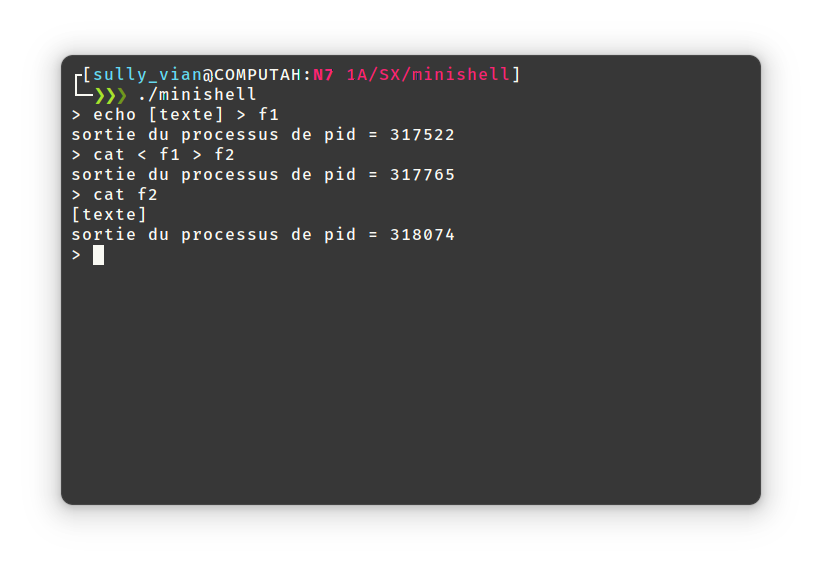
\includegraphics[width=\textwidth]{./resources/E16.png}
    \caption{Test de la redirection de l'entrée et de la sortie}
\end{figure}

Le texte \texttt{[texte]} est bien écrit dans \texttt{f1} à la première commande, puis, le contenu de \texttt{f1} est écrit dans \texttt{f2} à la deuxième commande. La troisième commande vérifie que le contenu de \texttt{f2} est bien celui prévu.

\subsection*{Étape 17 (Rendus 2)}
\addcontentsline{toc}{subsection}{Étape 17 (Rendus 2)}

Rien à faire.

\subsection*{Étape 19 (Tubes simples)}
\addcontentsline{toc}{subsection}{Étape 19 (Tubes simples)}

Voir l'étape 20.

\subsection*{Étape 20 (Pipelines)}
\addcontentsline{toc}{subsection}{Étape 20 (Pipelines)}

Une pipeline est une liste de commandes séparées par des tubes (\texttt{|}). La sortie de chaque commande est redirigée vers l'entrée de la commande suivante. Pour implémenter cela, il suffit de savoir si la commande actuelle est la première ou la dernière du pipeline et de mémoriser les descripteurs de fichier du tube d'une commande à l'autre.

Il est facile de savoir si une commande est la dernière d'un pipeline, le champ \texttt{seq} de \texttt{struct cmdline} se termine toujours par \texttt{NULL}. On teste donc la nullité de la commande suivante.

En revanche, pour savoir si une commande est la première d'un pipeline, j'ai introduit une nouvelle variable entière \texttt{dernier\_lu}. Cette variable garde en mémoire le descripteur de fichier de la sortie de la commande précédente.

Avec ces deux informations, il est facile de chainer les commandes entre elles, en remplaçant simplement les entrées / sorties des commandes par les descripteurs de fichier des tubes de la même manière que pour les redirections de l'étape 16.

\begin{lstlisting}[language=C, caption=gestion des pipelines]
while((cmd = commande->seq[indexseq])) {
    // tant qu'on n'est pas a la fin du pipeline
    /* ... */
    else {
        int tube[2];
        if (commande->seq[indexseq + 1] != NULL) {
            // s'il y a une commande suivante, creer un tube
            safepipe(tube);
        }
        switch (pid_fils = fork()) {
            /* ... */
            case 0: /* code du fils */
                /* ... */
                // redirection des tubes
                if (dernier_lu != -1) {
                    // si ce n'est pas la premiere commande, fixer l'entree standard a la sortie du tube precedent et fermer la sortie du tube
                    safedup2(dernier_lu, STDIN_FILENO, "in");
                    safeclose(dernier_lu, "in");
                }
                if (commande->seq[indexseq + 1] != NULL) {
                    // si ce n'est pas la derniere commande, fixer la sortie standard a l'entree du tube et fermer l'entree du tube
                    safeclose(tube[0], "dernier_lu2");
                    safedup2(tube[1], STDOUT_FILENO, "tube[1]");
                    safeclose(tube[1], "dernier_lu3");
                }
                /* ... */
                break;
            default: /* code du pere */

                if (dernier_lu != -1) {
                    // si un tube est ouvert, le fermer (le pere n'en a pas besoin)
                    safeclose(dernier_lu, "dernier_lu4");
                }
                if (commande->seq[indexseq + 1] != NULL) {
                    // s'il y a une commande suivante, fermer la sortie (pas besoin dans le pere)
                    safeclose(tube[1], "dernier_lu5");
                    // sauvegarder la sortie du tube pour la prochaine commande
                    dernier_lu = tube[0];
                }
                /* ... */
        }
    }
}
\end{lstlisting}

Dans la figure 9, on voit un exemple de pipeline avec les commandes \texttt{cat}, \texttt{grep} et \texttt{wc -l}. On compte le nombre de lignes de \texttt{minishell.c} contenant le mot \texttt{int}. \texttt{cat} affiche le contenu du fichier, \texttt{grep} filtre les lignes contenant le mot \texttt{int} et \texttt{wc -l} compte le nombre de lignes.

\begin{figure}[H]
    \centering
    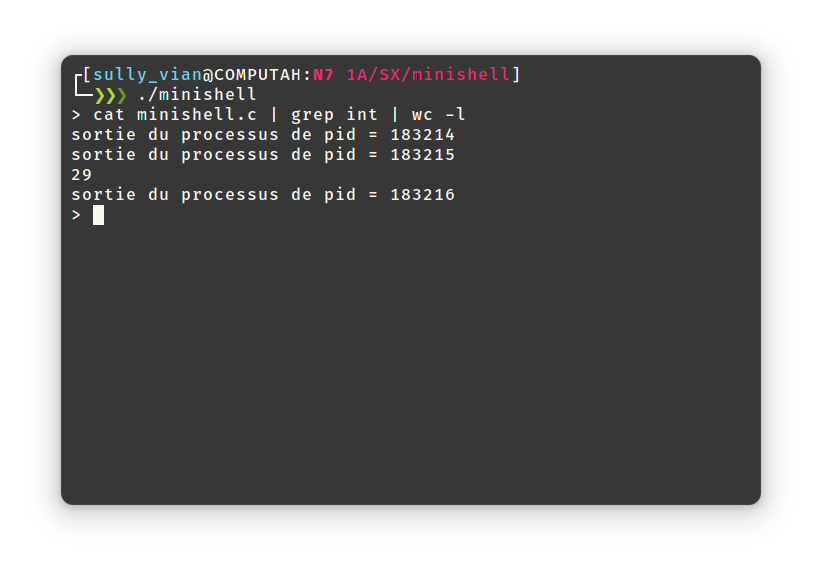
\includegraphics[width=\textwidth]{./resources/E20.png}
    \caption{Test d'un pipeline}
\end{figure}

On compte donc 29 lignes différentes contenant au moins une fois le mot \texttt{int} dans le fichier \texttt{minishell.c}. On remarque aussique les deux premières commandes s'arrètent avant l'affichage du résultat. C'est cohérent avec l'implémentation réalisée.

\subsection*{Étape 21 (Rendu)}
\addcontentsline{toc}{subsection}{Étape 21 (Rendu)}

Rien à faire.

\section{Codes complémentaires}

Dans le sujet, il nous est demandé de réaliser des codes complémentaires. J'ai placé ces codes dans le dossier \texttt{complement}.

\subsection{\texttt{copier.c}}

Ce pogramme est équivalent à la commande \texttt{cp} de Unix. Il se déroule en 3 étapes:

\begin{enumerate}
    \item ouvrir le fichier source en lecture seule et le fichier destination en écriture seule.
    \item boucler pour lire le contenu du fichier source fragment par fragment (de taille \texttt{BUFSIZE}) et écrire le fragment dans le fichier destination. Cette boucle s'arrête lorsqu'il n'y a plus rien à lire.
    \item fermer les fichiers source et destination.
\end{enumerate}

\subsection{\texttt{tube1.c}}

Ce programme ne peut pas fonctionner car le fils ne connait pas le tube créé par le père. Le fils a un descripteur de fichier identique à celui du père au moment du fork, mais ces copies de sont pas partagées.

\subsection{\texttt{tube2.c}}

Ce programme fonctionne correctement, le fils affiche bien l'entier écrit par le père.

\subsection{\texttt{tube3.c}}

Ce programme ne fonctionne pas comme espéré. Le père n'écrit plus dans le tube donc lefils n'a plus rien à y lire. Or, \texttt{read} est bloquant. Le fils reste donc bloqué dans la boucle. Le père non plus ne s'arrête pas car il attend un signal (\texttt{pause}).

\subsection{\texttt{tube4.c}}

Cette fois, le porgramme se termine bien parce que le père se termine après 10 secondes. En revanche, le fils n'affiche toujours pas de message puisque read est toujours bloquant. Il reste encore coincé dans la boucle.

\subsection{\texttt{tube5.c}}

\end{document}